La definición del error cuadrático medio es:
\begin{displaymath}
	ECM(\hat{\theta}) = V(\hat{\theta}) + Sesgo(\hat{\theta})^2
\end{displaymath}

Sabremos de antemano que el \textbf{E.C.M.} del estimador de momentos no será cero porque sus sesgos no son nulos. Sin embargo, el \textbf{E.C.M.} de los estimadores de la doble mediana y de máxima verosimilitud pueden llegar a serlo si $\lim_{n \to \infty} V(\hat{b}) = 0$.

\vskip 8pt

A continuación presentamos los errores cuadráticos medios para cada estimador en función de $n$, con $n$ siendo la cantidad de muestras de tamaño $15$:

\begin{figure}[H]
	\centering
	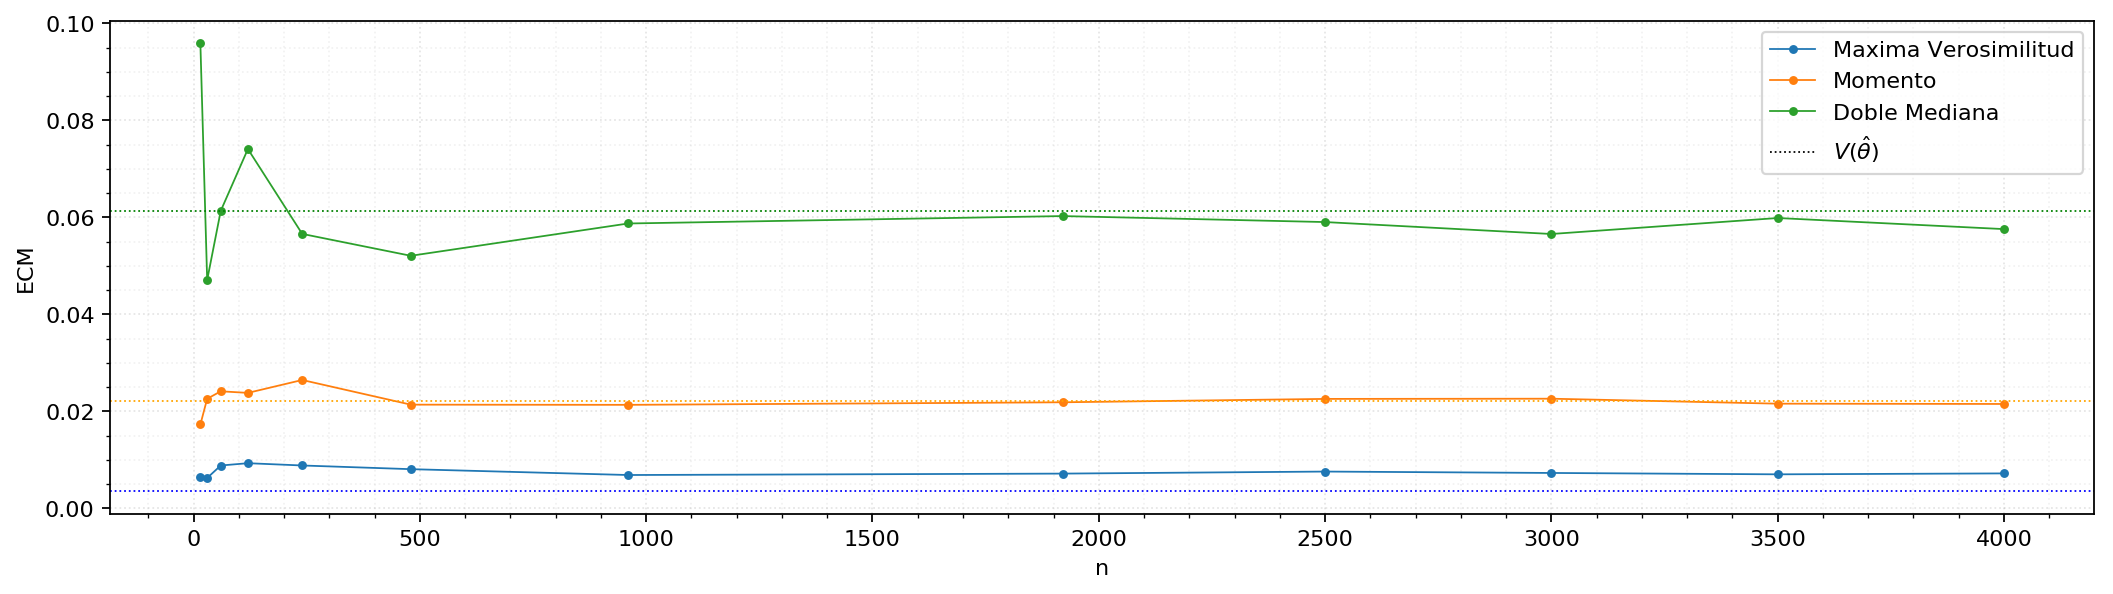
\includegraphics[width=1\textwidth]{imagenes/ecm-en-f-de-n-infinito.png}
	\caption{\footnotesize ECM de los estimadores en función de n. $a=0, b=1$}
	\label{fig:ej7-ecm-en-f-de-n}
\end{figure}

La figura \ref{fig:ej7-ecm-en-f-de-n} sugiere que el error cuadrático medio de los estimadores $\hat{b}_{mom}$ y $\hat{b}_{med}$ no tienden a cero. Sin embargo, el estimador de máxima verosimilitud muestra una significativa evidencia de tendencia al valor nulo. Por esta razón, tenemos razones para creer que su Error Cuadrático Medio tiende a cero a medida que se aumenta el valor de $n$. Veamos qué implicancias tiene:
\begin{align*}
	\lim_{n \to \infty} ECM(\hat{b}_{mv}) &= \lim_{n \to \infty} V(\hat{b}_{mv}) + Sesgo(\hat{b}_{mv})^2 \\
										  &= \lim_{n \to \infty} V(\hat{b}_{mv}) \text{ (porque asint. insesgado)} \\
										  &= 0
\end{align*}
Por lo tanto, se tiene que:
\begin{align*}
	\lim_{n \to \infty} V(\hat{b}_{mv}) = 0
\end{align*}

Al tener varianza cero y ser asintóticamente insesgado, el estimador cumple todas las hipótesis de consistencia. Además, por presentar la menor varianza de los estimadores insesgados, el principio de estimación insesgada de mínima varianza nos asegura que $\hat{b}_{mv}$ es el estimador que provee la mejor calidad de los tres.